\section{Algorithmic Components}
\label{sec:algorithmic-components}

\subsection{Instrument Signature Removal}
\label{sec:acISR}
AUTHOR: Merlin
\begin{itemize}
\item Mask defects and saturation
\item Assembly
\item Overscan
\item Linearity
\item Crosstalk
\item Full frame corrections: Dark, Flats (includes fringing)
\item Pixel level corrections: Brighter fatter, static pixel size effects
\item Interpolation of defects and saturation
\item CR rejection
\item Generate snap difference
\item Snap combination
\end{itemize}

\subsubsection{AP: just skip some steps?}
AUTHOR: Simon
\begin{itemize}
\item Indicate steps to be done by camera
\item call out other steps that are omitted/modified relative to the DRP version
\end{itemize}

\subsubsection{DRP: do all the steps}
AUTHOR: Merlin


\subsection{Artifact Detection}
\label{sec:artifact}

\subsubsection{Single-Exposure Morphology}
\label{sec:acMorphologicalArtifactDetection}
\paragraph{Cosmic Ray Identification}
Cosmic rays will be identified using a Laplacian edge detection algorithm \citep{dokkum01}.  Laplacian edge detection involves convolving the image (I) with a smoothing function (f) tuned to the size of the expected edge width.
\[
L = \bigtriangledown^2f\ast I
\]
In the case of cosmic rays, this implies a very sharp edge.  A natural choice is a Gaussian with small $\sigma$.  The discrete kernel chosen in \citep{dokkum01} is
\begin{align}
\bigtriangledown^2 = \frac{1}{4}\left( \begin{array}{ccc}
0 & -1 & 0 \\
-1 & 4 & -1 \\
0 & -1 & 0 \end{array} \right)
\end{align}
If just used on the native image, this filter would attenuate the signal from CRs that effect multiple adjacent pixels.  So, the image is subsampled by some factor $f_s$.  The before downsampling to the native resolution, the negative pixel values are clamped to zero.  The resultant image in native pixelization will be referred to as $L^+$.

We construct a SNR image by dividing the Laplacian image by the noise in the image and adjusting by the subsampling factor.
\[
S = \frac{L^+}{f_s N}
\]

This CR detection image can be cleaned further by removing extended sources using a median filter. $M_n$ is the median over a $n \times n$ box.
\[
S^\prime = (S \ast M_5)
\]
If the PSF is well sampled, this SNR image can be used to detect the CRs by simply drawing a threshold in SNR.  If the PSF is undersampled, the author uses the assumption that undersampled point sources are more symmetric than CRs.  By constructing a "fine-structure" image, one can plase a minimum contrast between the Laplacian image and the fine structure image that further improves differentiation between CRs and point sources.
\[
F = (M_3 \ast I) - [(M_3 \ast I) \ast M_7]
\]

So the final CR selection criteria are: $S^\prime > \sigma_{lim}$ and $L^+/F > F_{lim}$.  The tuning parameters are: $f_s$ the subsampling rate, $\sigma_{lim}$ the SNR of the CRs in the detection image, $f_{lim}$ the minimum contrast relative to the "fine-structure" image.

\begin{note}[Add to SFM section]
We can use something like L.A.COSMIC (or CRBLASTER) but if it is too slow, we can fall back to the SDSS algorithm which does a similar thing, but does no convolutions.
We should also consider why we do not use a Canny algorithm instead.
\end{note}
\paragraph{Optical ghosts}
We will have a set of optical ghost models.  Some of these will be models of stationary ghosts (e.g. pupil ghost). Others will be a set of ghosts produced by point sources as a function of source position and brightness. The latter will likely be modeled using tools like ZEMAX or measured using projectors.

The stationary ghosts will need to be fit for since they will depend on the total light through the pupil rather than on the brightness of a given source and we do not expect to have the data necessary to compute the total flux over the focalplane in a single thread in the alert production processing.  Using the fit to stationary models $S$ and the predictions of the single source ghosts, $P$, we will constructy a ghost image
\[
I_g = \Sigma_i S_i + \sigma_j P_{j}
\]
where $i$ runs over the stationary ghost models and $j$ runs over the sources contributing to single source ghosts.  We can then correct the image by:
\[
I^\prime = I - I_g
\]

\begin{note}[dependence on PSF]
The CR rejection algorithm does not depend on the PSF of the image.  The single source ghosts may be a function of the PSF, but not very strongly I don't think.
\end{note}

\subsubsection{Single-Exposure Aggregation}
\paragraph{Linear feature detection and removal}
Satellite trails, out of focus airplanes, and meteors all cause long linear features in astronomical images.  The Hough Transform \citep{citation_needed} is a common tool used in computer vison applications to detect linear features.  Linear features are parameterized by $r$, the perpendicular distance to the line from the origin and $\theta$, the the angle of $r$ with the x-axis.  The $(r, \theta)$ space is binned and each pixel in the image adds its flux to all the bins consistent with that pixel location.  For bright linear features, the bin at the true location of the feature will fill up because more than one bright pixel is contributing to that location in parameter space.  After all pixels have been polled, the highest bins correspond to the linear features in the image.

This works very well in high signal-to-noise images, but is very computationally expensive.  It is also susceptible to bright point sources overwhelming faint linear features.  

An algorithm that takes care of both of these issues is presented in \cite{borncamp_lim16}.  We will use this as our baseline.  First the image is rescaled to bring out faint features.  Next an edge detectionalgorithm is run on the image.  The reference implementation uses a Canny algorithm \citep{canny86}.  This algorithm produces a set of edges that can then be mined for linear features.  They use a probababalistic Hough Transforms \citep{galambos99} to cut down on computational costs.  The probabalistic version limits the number of pixels that vote.  This results in a list of line segments.  The segments are binned in angle and any sement that is outside some tolorance of the mode is culled.  This cleaned set of segments is fed to the masking algorithm.

The masking algorithm traverses each line segment found in the previous step by selecting a subregion around the segment and flattening the subregion.  A weighted mean of the subregion is computed and any pixels above some threshold are considered part of the trail and masked.  The subregion is moved along the segment until the end is reached.  This is repeated for every segment.

One of the assumptions of the algorithm is that the trail crosses the whole image.  I don't think we want to make that assumption.  I also don't know why they run a Canny algorithm first and then do a Hough Transform.  I guess it does the same sort of regularization that Steve tried to do with his moments.

\begin{note}[Bickerton writeup]
Note that there is a writeup by Steve Bickerton on a different way to modify the Hough Transform to find satelite trails and it has been tried on HSC, but the paper is not complete.  Thus, I didn't use it as the baseline here.  The writeup is linked from DM-5872.
\end{note}

\subsubsection{Snap Subtraction}
\label{sec:acSnapSubtraction}
\paragraph{Improvements by using multiple snaps}
{\bf Cosmic Rays}
We will need to still run some sort of topological identifier like the one outlined above.  This is because there will be real transients and we still only want to pick out the sharp features as CRs.  It will help to have less crowding, so we should do CR rejection on the snap difference if we have it.

{\bf Ghosts}
Snap differences will not help with ghosting as the ghosts should difference almost perfectly.

{\bf Linear features}
Snap differences will provide significant leverage for masking linear features.  Since each segment will appear in at most one snap we can mask based on the pixels marked as detected in the difference images that are part of the trail.  This will help in crowded regions.  This technique will require running some sort of trail detection algorithm, but the requirements will be less stringent since the image will be so much less crowded.

\subsubsection{Warped Image Comparison}
\label{sec:acWarpedImageArtifactDetection}
AUTHOR: Jim
\begin{itemize}
\item Find more optical artifacts by looking at differences between warped images (this is run during background matching).
\item Find transient astronomical sources we don't want to include in coadds.
\end{itemize}

\subsection{Artifact Interpolation}
\label{sec:acArtifactInterpolation}
AUTHOR: Jim
\begin{itemize}
\item Set mask planes for all artifacts.
\item Eliminate small artifacts by interpolating them.
\item Uses PSF model as interpolant.
\end{itemize}

\subsection{Source Detection}
\label{sec:acSourceDetection}
AUTHOR: Jim
\begin{itemize}
\item Detect above-threshold regions and peaks in direct or difference images.
\item Needs to work on preconvolved and unconvolved images.
\item May need multi-pass variants: detect bright objects first, then faint; detect with approximate PSF, then improved.
\item Need to work on wavefront sensors (with out-of-focus PSFs)
\end{itemize}

\subsection{Deblending}
\label{sec:acDeblending}
AUTHOR: Jim

For templates, try:
\begin{itemize}
\item symmetry ansatz with additional regularization
\item simultaenous fit of galaxy models
\item spline-based models with regularization?
\item (multi-coadd only) optimize color uniformity
\end{itemize}

Will be especially challenging in crowded fields, but it needs to work in that regime as well.

\subsubsection{Single Frame Deblending}
\label{sec:acSingleFrameDeblending}
\begin{itemize}
\item Generate HeavyFootprint deblends using only a single image.
\item May need to be able to work with approximate/guess PSF, even in crowded fields, if we need to deblend before PSF estimation in DRP.
\item May need to work on wavefront sensors (with out-of-focus PSFs)
\end{itemize}

\subsubsection{Multi-Coadd Deblending}
\label{sec:acMultiCoaddDeblending}
\begin{itemize}
\item Generate consistent HeavyFootprint deblends from coadds over multiple bands and possibly epoch ranges.
\end{itemize}

\subsection{Measurement}
\label{sec:acMeasurement}
AUTHOR: Jim

\begin{figure}
\centering
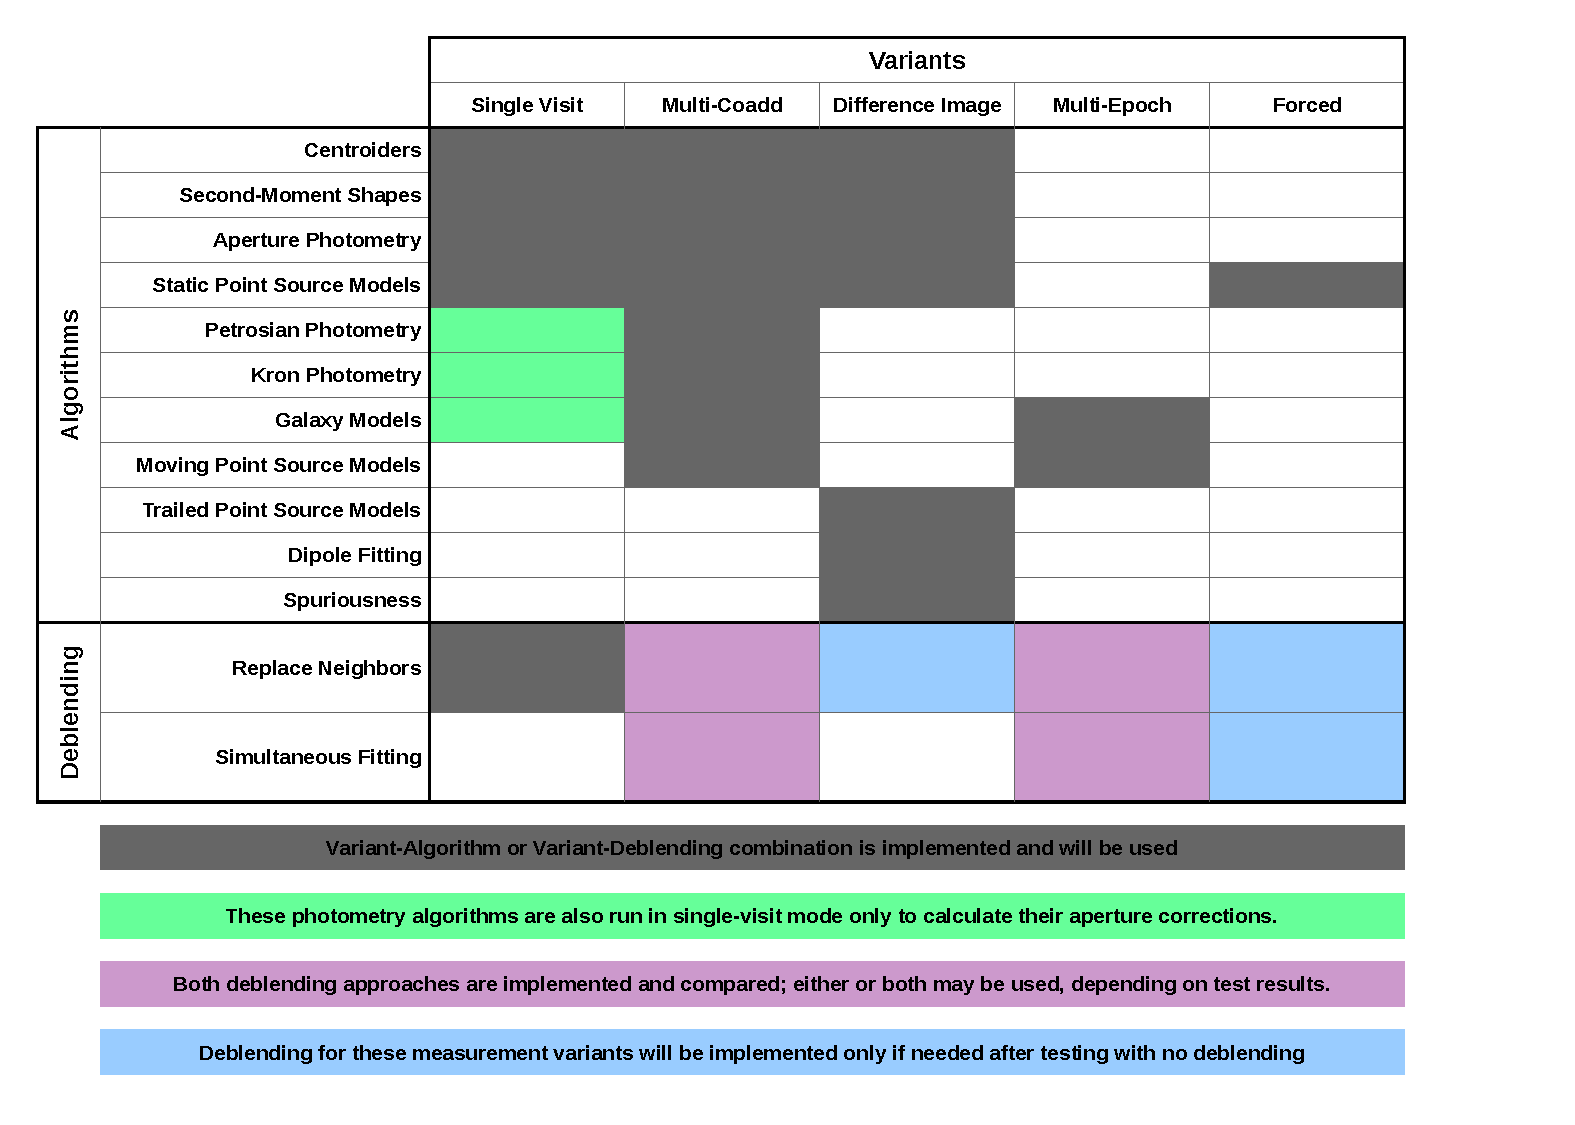
\includegraphics[width=\textwidth]{figures/measurement-matrix.pdf}
\caption{Matrix showing combinations of measurement variants, algorithms, and deblending approaches that will be implemented.
\label{fig:measurement-matrix}}
\end{figure}

\subsubsection{Variants}
Measurement is run in several contexts, but always consists of running an ordered list of algorithm plugins on either individual objects or families thereof.  Each context corresponds to different variant of the measurement driver code, and has a different set of plugin algorithms and approaches to measuring blended objects.

\paragraph{Single Frame Measurement:} Measure a direct single-visit CCD image, assuming deblend information already exists and can be used to replace neighbors with noise (see \ref{sec:acReplaceNeighborsWithNoise}).
\label{sec:acSingleFrameMeasurement}

Single Frame Measurement is run in both \hyperref[sec:apSingleFrameProcessing]{AP's Single Frame Processing pipeline}) and DRP's \hyperref[sec:drpBootstrapImChar]{BootstrapImChar}, \hyperref[sec:drpRefineImChar]{RefineImChar}, and \hyperref[sec:drpFinalImChar]{FinalImChar}.  It must be capable of running on wavefront sensor images, though this may require different plugin algorithms.

The driver for Single Frame Measurement is passed an input/output \hyperref[sec:spTablesSource]{SourceCatalog} and an \hyperref[sec:spImagesExposure]{Exposure} to measure.  Plugins take an input/output \hyperref[sec:spTablesSource]{SourceRecord} and an \hyperref[sec:spImagesExposure]{Exposure} containing only the object to be measured.

\paragraph{Multi-Coadd Measurement:} Simultaneously measure a suite of coadds representing different bandpasses, epoch ranges, and flavors.  This is run only in DRP's \hyperref[sec:drpMeasureCoadds]{MeasureCoadds} pipeline.
\label{sec:acMultiCoaddMeasurement}

The driver for Multi-Coadd Measurement is passed an input/output \hyperref[sec:spTablesObject]{ObjectCatalog} and a dict of \hyperref[sec:spImagesExposure]{Exposures} to be measured.  Plugins take an input/output \hyperref[sec:spTablesObject]{ObjectRecord} and a dict of \hyperref[sec:spImagesExposure]{Exposures}, each containing only the object to be measured.  Some plugins will also support simultanous measurement of multiple objects, which requires they be provided the subset of the \hyperref[sec:spTablesObject]{ObjectCatalog} to be measured and a dict of \hyperref[sec:spImagesExposure]{Exposures} containing just those objects.

\paragraph{Difference Image Measurement:} Measure a difference image, potentially using the associated direct image as well.  Difference image measurement is run in AP's \hyperref[sec:apAlertDetection]{Alert Detection} pipeline and DRP's \hyperref[sec:drpDiffIm]{DiffIm} pipeline.
\label{sec:acDiffImMeasurement}

The signatures of difference image measurement's drivers and algorithms are at least somewhat TBD; they will take at least a difference image \hyperref[sec:spImagesExposure]{Exposures} and a \hyperref[sec:spTablesSource]{SourceCatalog/SourceRecord}, but some plugins such as dipole measurement may require access to a direct image as well.  Because difference imaging dramatically reduces blending, difference image measurement may require any approach to blended measurement (though any use of the associated direct image would require deblending).

If preconvolution is used to construct difference images, but they are not subsequently decorrelated, the algorithms run in difference image measurement cannot be implemented in the same way as those run in other measurement variants, and algorithms that cannot be expressed as a PSF-convolved model fit (such as second-moment shapes and all aperture fluxes) either cannot be implemented or require local decorrelation.

\paragraph{Multi-Epoch Measurement:} Measure multiple direct images simultaneously by fitting the same \hyperref[sec:spWCS]{WCS}-transformed, \hyperref[sec:spPSF]{PSF}-convolved model to them.  Blended objects in Multi-Epoch Measurement will be handled by \emph{at least} fitting them simutaneously (\ref{sec:acSimultaneousFitting}), which may in turn require hybrid galaxy/star models (\ref{sec:acHybridModels}).  These models may then be used as templates for deblending and replace-with-noise (\ref{sec:acReplaceNeighborsWithNoise}) measurement if this improves the results.
\label{sec:acMultiEpochMeasurement}

Because the memory and I/O requirements for multi-epoch measurement of a single object or blend family are substantial, we will not provide a driver that accepts an \hyperref[sec:spTablesObject]{ObjectCatalog} and measures all objects within it; instead, the \hyperref[sec:drpMultiFit] pipeline will submit individual family-level jobs directly to the orchestration layer.  The multi-epoch measurement driver will thus just operate on one blend family at a time, and manage blending while executing its plugin algorithms.

Multi-epoch measurement for DRP only includes two plugin algorithms, so it is tempting to simply hard-code these into the driver itself, but this driver will also need to support new plugins in Level 3.

Multi-epoch measurement will also be responsible for actually performing forced photometry on direct images, which it can do by holding non-amplitude parameters for moving point-source models fixed and adding a new amplitude parameter for each observation.

\paragraph{Forced Measurement:} Measure photometry on an image using positions and shapes from an existing catalog.
\label{sec:acForcedMeasurement}

In the baseline plan, we assume that forced measurement will only be run on difference images; while forced photometry on direct images will also be performed in DRP, this will be done by multi-epoch measurement.

Because difference imaging reducing blending substantially, forced measurement may not require any special handling of blends.  If it does, simultaneous fitting (with point-source models) should be sufficient.

The driver for Forced Measurement is passed an input/output \hyperref[sec:spTablesSource]{SourceCatalog}, an additional input \hyperref[sec:spTablesReference]{ReferenceCatalog}, and an \hyperref[sec:spImagesExposure]{Exposure} to measure.  Plugins take an input/output \hyperref[sec:spTablesSource]{SourceRecord}, an input \hyperref[sec:spTablesReference]{ReferenceRecord} and an \hyperref[sec:spImagesExposure]{Exposure}.  If simultaneous fitting is needed to measure blends, plugins will instead receive subsets of the catalogs passed to the driver instead of individual records.

Forced measurement is used by the DRP \hyperref[sec:drpForcedPhotometry]{ForcedPhotometry} pipeline and numerous pipelines in AP.

\begin{note}[TODO]
Add references to specific AP pipelines that will use forced measurement.
\end{note}

\subsubsection{Algorithms}

\paragraph{Centroids}
\label{sec:acCentroidAlgorithms}
\begin{itemize}
\item should be equivalent to PSF model fit for stars
\item use larger weight function (TBD) for extended objects
\item need variant that doesn't require a PSF model (or can work with a poor guess) to run before PSF estimation.
\item need to have a version (possibly the main version) that works on wavefront sensors
\end{itemize}

\paragraph{Pixel Flag Aggregation}
\label{sec:acPixelFlags}
\begin{itemize}
\item Compute summary statistics of masked pixels in the neighborhood of the source/object.
\end{itemize}

\paragraph{Second-Moment Shapes}
\label{sec:acShapeAlgorithms}
\begin{itemize}
\item probably adaptive elliptical Gaussian weights, with fall back to unweightd, PSF-weighted, or some fixed Gaussian
\item add regularization for unresolved objects - avoid crazy ellipticities for objects much smaller than PSF
\item Should also compute moments of PSF model.
\item Need to have a version (possibly the main version) that works on wavefront sensors to characterize the donut-like out-of-focus sources.
\end{itemize}

\paragraph{Aperture Photometry}
\label{sec:acAperturePhotometry}

\begin{itemize}
\item Aperture fluxes are computed by summing the total flux within an elliptical region defined on the image.
\item Aperture fluxes are computed at a series of logarithmically spaced aperture sizes. Per the \DPDD{}, the total number of apertures will vary depending on the size of the source.
\item When computing fluxes for small apertures---for configurable values of ``small''--we use $\mathrm{sinc}$ interpolation \cite{Bickerton13}. For large apertures, we use a naive summation of pixel values.
\item May need to change ellipticity as a function of aperture radius.
\item If run before PSF estimation, will need a variant that does not rely on the PSF model to choose aperture size/ellipticity.
\end{itemize}

\paragraph{Static Point Source Models}
\label{sec:acStaticPointSourceModels}
\begin{itemize}
\item Fit PSF model for flux only (hold center fixed at centroid or reference value)
\item Doesn't use per-pixel variances for flux measurement, but might also provide measurement with per-pixel variances (for diagnostics?)
\end{itemize}

\paragraph{Kron Photometry}
\label{sec:acKronPhotometry}
\begin{itemize}
\item Compute Kron radius (hard to make this robust)
\item Compute flux in elliptical aperture at Kron radius.
\end{itemize}

\paragraph{Petrosian Photometry}
\label{sec:acPetrosianPhotometry}
\begin{itemize}
\item Compute Petrosian radius.  Harder than it seems due to need for improvements to splines? (ask RHL)
\item Compute flux in elliptical aperture at Petrosian radius.
\end{itemize}

\paragraph{Galaxy Models}
\label{sec:acGalaxyModels}
\begin{itemize}
\item Some sort of bulge+disk model.  Lots of need for experimentation.
\item Will Monte Carlo sample in MultiFit (and maybe on coadds, too, if that helps).
\item May also fit to PSF-matched coadds for consistent colors.
\item Will need to support simultaneous fitting (and sampling).
\item Hybrid model candidate
\end{itemize}

\paragraph{Moving Point Source Models}
\label{sec:acMovingPointSourceModels}
\begin{itemize}
\item Fit point source with flux, centroid, parallax, and proper motion parameters.
\item May need to support simultaneous fitting.
\item Might want to sample this too, at least if we fit it simultaneously with sampled galaxy models.
\item Hybrid model candidate
\end{itemize}

\paragraph{Trailed Point Source Models}
\label{sec:acTrailedPointSourceModels}
\begin{itemize}
\item Fit PSF convolved with line segment to individual images
\end{itemize}

\paragraph{Dipole Models}
\label{sec:acDipoleModels}
\begin{itemize}
\item Fit PSF dipole for separation and flux to a combination of difference image and direct image.
\item Deblending on direct image very problematic.
\end{itemize}

Arising primarily due to slight astrometric alignment or PSF matching errors between the two images, or effects such as differential chromatic aberration, flux “dipoles” are a common artifact often observed in image differences. These dipoles will lead to false detections of transients unless correctly identified and eliminated. Importantly, dipoles will also be observed in image differences in which a source as moved less than the width of the PSF. Such objects must be correctly identified and measured as dipoles in order to obtain accurate fluxes and positions of these objects. 

Putative dipoles in image differences are identified as a positive and negative source whose footprints overlap by at least one pixel. These overlapping footprints are merged, and only the sources containing one and only one positive and negative merged footprint are passed to the dipole modeling task. There is a documented degeneracy (\url{http://dmtn-007.lsst.io}) between dipole separation and flux, such that dipoles with closely-separated lobes of high flux are statistically indistinguishable from ones with low flux and wider separations. We remove this degeneracy by using the {\em pre-subtracted images} (i.e., the warped, PSF-matched template image and the pre-convolved science image) to constrain the lobe positions (specifically, to constrain the centroid of the positive lobe in the science image and of the negative lobe in the template image). This is done by first fitting and subtracting a second-order 2-D polynomial to the background within a subimage surrounding each lobe footprint in the pre-subtracted images to remove any flux from background galaxies (we assume that this gradient, if it exists, is identical in both pre-subtracted images). Then, a dipole model is fit simultaneously to the background-subtracted pre-subtracted images and the image difference. 

The dipole model consists of positive and negative instances of the PSF in the difference image at the dipole's location. The six dipole model parameters (positive and negative lobe centroids and fluxes) are estimated using non-linear weighted least-squares minimization (we currently use the Levenberg-Marquardt minimization algorithm). The resulting reduced $\chi^2$ and signal-to-noise estimates provide a measure by which the source(s) may be classified as a dipole. 

We have tested the described dipole measurement algorithm on simulated dipoles with a variety of fluxes, separations, background gradients, and signal-to-noise. Including the pre-subtracted image data clearly improves the accuracy of the measured fluxes and centroids. We have yet to thoroughly assess the dipole measurement algorithm performance on crowded stellar fields. Such crowded fields may confuse the parameter estimates (both centroids and/or fluxes) when using the pre-subtracted images to constrain the fitting procedure, and in such situations, we may have to adjust the prior constraint which they impose. 

\paragraph{Spuriousness}
\label{sec:acSpuriousnessAlgorithms}
\begin{itemize}
\item Some per-source measure of likelhood the detection is junk (in a difference image).
\item May use machine learning on other measurements or pixels.
\item May be augmented by spuriouness measures that aren't purely per-source.
\end{itemize}

\subsubsection{Blended Measurement}
\label{sec:acBlendedMeasurement}
\begin{itemize}
\item Integrate text from blended-measurement doc here.
\end{itemize}

\paragraph{Deblend Template Projection}
\label{sec:acDeblendTemplateProjection}
\paragraph{Neighbor Noise Replacement}
\label{sec:acReplaceNeighborsWithNoise}
\paragraph{Simultaneous Fitting}
\label{sec:acSimultaneousFitting}
\paragraph{Hybrid Models}
\label{sec:acHybridModels}

\label{Spatial Models}
\label{sec:acSpatialModels}
In many areas we will need to represent spatial models.  This will include models fit to sparse and non-uniformly sampled data.  We will support fitting Chebyshev polynomials and splines.  We will also support regression techniques like Gaussian Processes.

\subsection{Background Estimation}
\label{sec:acBackgroundEstimation}

Background estimation will be done on the largest scale feasible first.  In the case of Alert Production, this may be on the size of a chip.  In DRP, we expect this to be on a full focalplane.  An initial low order estimate will be made on a large scale.  Each chip will be divided into subregions.  For each subregion, the median of the non-masked pixels will be computed.  All values for all chips will be fit by an appropriate function (see \S \ref{sec:acSpatialModels}).  This will provide a low order background estimation in focal plance coordinates.  Note that this can only be done if the instrument signature removal is very high fidelity.  Any sharp discontinuity could cause problems with fitting a smooth function.

A higher order background model can be computed per chip.  First, the low order background is subtracted from the image.  The non-masked pixels will again be binned on a finer grid avoiding bright objects.  The median in each bin is fit by an appropriate function.  In practice, this process will likely be iterative.

In the case of Alert Production, there will be no full focalplane model since we expect to process only a single chip in each thread.  In this case, we constrain the background with the available un-masked pixels without removing a global background first.  Note that image differencing is still possible even in the scenario where there are no unmasked pixels in the science image.  The background can be modeled as a part of the PSF matching process.  We will want to do background modeling and subtraction in Alert Production when possible because we will want to do calibrated photometry.  Even though these measurements are not persisted for science us, they will be very useful for debugging and QA.

If there are so few un-masked pixels in the entire focalplane that even a low order global background is impossible to model, we will not compute a background model.  Instead, we will do crowded field photometry only \ref{????}

\begin{note}[Crowded fields and composition]
Requirements included working in crowded fields.  I think estimating a full focalplane model is the best we can do.  If there are no unmasked pixels in the entire FoV, I don't think there is much we can do.
I didn't explicitly talk about composition of background models, but this takes that into account by allowing a global model to be subtracted from the single chip image before a higher order model is fit.
\end{note}

\subsection{Build Background Reference}
\label{sec:acBuildBackgroundReference}
AUTHOR: Simon
\subsubsection{Patch Level}
Background-matching each \texttt{CoaddTempExp} (CTE) to a reference exposure performs comparably to fitting
the offsets to the N(N-1)/2 difference images, however the co-add quality will depend on the quality of the
reference image.  Choosing a reference image on a per-patch basis is as simple as choosing the CTE that
maximizes both coverage and the SNR of the sky background. Coverage is defined as the fraction of non-NaN
pixels in the CTE. NaN pixels arise in CTEs because of gaps between the chips and edges of the visit focal
planes.  The camera design specifications indicate a 90\% fill factor, and thus approximately 10\% of pixels
will be NaN due to chip gaps.  The SNR of the background can be estimated from either the CTEs themselves,
using the variance plane of pixels without the source detection bit mask flagged, or from calibration
statistics such as the zero point (a proxy for transparency).  In the limiting case that all CTEs have the
same coverage, finding the best reference image reduces to the problem of weighting epochs in co-addition.
For example, the reference image that minimizes the variance in the co-add is the minimum variance CTE, and
the reference image that maximizes SNR in coadd point source measurements is the CTE with the maximum
$T_i/{\rm FWHM}^2_i \sigma^2_i$\footnote{to the first order. Don't want to start a fight here}, where $T_i$ is
the transparency,  and $\sigma^2_i$ the average variance of the pre-scaled exposure.  By combining one of
these statistics with coverage, we can construct an objective/cost function that relates the importance of
coverage and sky-background, and can select a visit that minimizes that quantity objective function.

\subsubsection{}
Constructing reference images for tract-sized co-adds follows the same principle, but requires maximizing the
SNR/coverage of a large mosaic constructed from multiple visits.  Algorithms for mosaicking partially
overlapping images have been well established \citep[e.g.][]{Sick2013, Berriman2008}. By mosaicking visits,
applying additive scalar or sloping offsets to calexps, we can generate a tract-sized reference image.
Algorithms for selecting visits to construct these fall on a spectrum of computational expense. On the less
expensive side is a greedy algorithm which starts with a ``best'' (as defined above) visit chosen at the
center of the tract.  Visits can be chosen, scaled, and added one by one in the vicinity, moving outwards.  A
another option is to choose a small set of visits that completely cover a tract without gaps, which can be
cast as a constrained convex optimization problem\footnote{probably}, and mosaic them using standard
mosaicking techniques.  Finally, the most expensive option would use all the visits to simultaneously tie the
visits together using all overlaps while background matching.

\begin{itemize}
\item Given multiple overlapping visit images (already warped to a common coordinate system), synthesize a continuous single-epoch image that can be used as a reference for background matching.
\end{itemize}

\subsection{PSF Estimation}
\label{sec:acPSFEstimation}

\subsubsection{Single CCD PSF Estimation}
\label{sec:acSingleCCDPSF}

Single CCD PSF estimation needs to be run in both Alert Production and in in Data Release Processing.  In Alert Production it will be the final PSF model for both direct and difference image measurement.  In Data Release Processing, it will be used as an initial bootstrapping step to start off image characterization.  We do not intend to include chromatic effects in the PSF at the single CCD estimation phase.

The first step is to select a set of suitable stars to use as PSF exemplars.  This can be done by finding clusters in second moment space.  In production, we expect that an external catalog with PSF candidates that have been show to be non-varying and isolated will produce better results.

Once a set of candidate stars is selected each star is fit by a set of appropriate basis functions: e.g. shapelets.  The PSF is approximated by
\[
P = \Sigma_n c_n\Psi_n
\]
where $\Psi_n$ is the $n^{th}$ basis function, and $c_n$ is the coefficient for that basis function.  We can solve for the coefficients in the least squares sense using a QR decomposition or similar technique.  We then have an estimate of the PSF at several locations on the chip.  For each of the coefficients we can fit 2D Chebyshev polynomials to each coefficient to model the spatial variation in each component (see \ref{sec:acSpatialModels}).  By interpolating the fit coefficients, we can derive an estimate of the PSF at any point in the chip.

The order of the spatial model cannot excede number of PSF exemplars in the frame.  If there is only a single PSF candidate star, we will assume the PSF is constant across the CCD.  In the case of no PSF candidate stars, we will assume a double Gaussian PSF with width set by observation metadata: e.g. FWHM from the guiding system.

\begin{note}[Do we need something more complex?]
We can get arbitrarily complex, but I don't thinkn we need a more complex system in the baseline until we show this won't work.
\end{note}

\subsection{Wavefront Sensor PSF Estimation}
\label{sec:acWavefrontSensorPSF}
AUTHOR: Jim
\begin{itemize}
\item Build an approximate PSF model using only the very brightest stars in the wavefront sensors.  Because WF sensors are out-of-focus, these stars may be saturated on science CCDs.
\item Model can have very few degrees of freedom (very simple optical model + elliptical Moffat/Double-Gaussian?)
\item Only needs to be good enough to bootstrap PSF model well enough to bootstrap processing of science images (but it needs to work in crowded fields, too).
\item Being able to go to brighter magnitudes may be important in crowded fields because the shape of the luminosity function may make it easier to find stars with (relatively) significant neighbors.
\end{itemize}

\subsubsection{Full Visit PSF Estimation}
\label{sec:acFullVisitPSF}
AUTHOR: Jim
\begin{itemize}
\item Decompose PSF into optical + atmosphere.
\item May also use wavefront sensors.
\item Constrain model with stars, telemetry, and wavefront data.
\item Wavelength-dependent.
\item Used in RefineImChar in DRP.
\item Must include some approach to dealing with wings of bright stars.
\end{itemize}

\subsection{Model Spatial Variation of PSF}
\subsubsection{Within a CCD}
\label{sec:acModelSpatialPSF}

\begin{itemize}
\item Estimate PSF at discrete locations using a set of basis functions
\item Fit interpolation functions to fit coefficients to enable interpolation
\end{itemize}
\subsubsection{Over a focal plane -- Do we need this?}

\subsection{Aperture Correction}
\label{sec:acApCorr}
AUTHOR: Jim
\begin{itemize}
\item Measure curves of growth from bright stars (visit-level, at least in DRP)
\item Correct various flux measurements to infinite (CCD-level)
\item Propagate uncertainty in aperture correction to corrected fluxes; covariance is tricky.
\end{itemize}

\subsection{Astrometric Fitting}
\label{sec:acAstrometricFitting}
AUTHOR: Simon
\subsubsection{Single CCD}
\label{sec:acSingleCCDAstrometricFit}
Used by AP, probably (RHL worries we might need full-visit)

AP will need to do reasonably good astrometeric calibration on single frames in order to do the relative warping between the template and science images.  We will use the internal reference catalog used in DRP as the reference catalog.  This will be based on astrometry from an external source and will be extended using high quality measurements on coadds from DRP.

We will use a matching algorithm like that outlined in \cite{tabur04}.  Once we match, a 2D polynomial solution will be fit to minimize the residual.

\begin{note}[Dependency]
This introduces a dependency on DRP's internal reference catalog not capture elsewhere.
\end{note}

\subsubsection{Single Visit}
\label{sec:acSingleVisitAstrometricFit}
Full visit astrometric fitting will be done as a bootstrapping step toward higher quality calibration in DRP.  All measurements in the visit will be projected to a tangent plane, taking into account all knowledge of the sensor arrangement and optics.  The reference catalog (likely the DRP reference catalog) will be projected to the same tangent plane.

Sources will be matched, again using a \cite{tabor04} like algorithm.  Once the reference and observations are matched, a multi-component WCS will be fit.  We expect the components will be related to residuals on the optical model and will included a component to account for the Von Karman turbulence.

\subsubsection{Joint Multi-Visit}
\label{sec:acJointAstrometicFit}
In the case where there are multiple visits overlapping the same part of the sky, e.g. a patch, we can leverage multiple realizations to beat down the random contribution of the atmosphere to get a better estimate of the optical model and the atmospheric contribution per visit.

The catalogs are stacked and matched using a multi-matching algorithm like OPTICS.  At this point, the measurements can be matched to an external catalog for the purposes of absolute astrometry.  With all measurementss in hand, a multi-component WCS is fit to all measurements at the same time on order to minimize the residual from the mean position for each object.

\subsection{Photometric Fitting}
\label{sec:acPhotometricFitting}
\subsubsection{Single CCD (for AP)}
\label{sec:acSingleCCDPhotometricFit}
\begin{itemize}
\item Match to photometric calibration reference catalog
\item Calculate single zeropoint using available color terms
\end{itemize}
\subsubsection{Single Visit}
\label{sec:acSingleVisitPhotometricFit}
\begin{itemize}
\item Fit zeropoint (and some small spatial variation?) to all CCDs simultaneously after matching to reference catalog.
\item Need for chromatic dependence unclear; probably driven by AP.
\item Might be possible to use a "nightly zeropoint" if calibration fields are taken (e.g., during twilight)
\end{itemize}



\subsubsection{Joint Multi-Visit}
\label{sec:acJointPhotometricFit}

For DRP, all the observations can be combined in the so-called ubercal procedure to generate the best possible measurement of the relative flux of each source. 

\begin{itemize}
\item Derive SEDs for calibration stars from colors and reference catalog classifications.
\item Utilize additional information from wavelength dependent photometric calibration built by calibration products production to convert observed flux to a flux through a standard atmosphere.
\item Fit zeropoint and possibly perturbations to all CCDs on multiple visits simultaneously after matching to reference catalog.
\end{itemize}

Because the number of stars gets ridiculously large, it can be useful to solve different overlapping regions of the sky in parallel.  Once all the regions converge, you can run the same ubercal matrix solution to tie the patches together.  The fist step is to solve:
\begin{equation} \label{eq:uber}
m_{ij} = m_i + z_j
\end{equation}
where $m_{ij}$ is an observed magnitude of star with true magnitude $m_i$ on observation $j$.  While it is possible to include more terms (say, fit out flat-fielding errors at the same time), more terms makes it much harder to solve in parallel.  Additional terms also make it easy to make the problem degenerate and it can slow the ubercal algorithm down rapidly. Naively, solving Equation~\ref{eq:uber} would involve simply computing the psudo-inverse of the sparse $m_{ij}$ matrix. Unfortunately, the inverse of a large sparse matrix is a large dense matrix.  Thus one must use iterative solvers such as the LSQR algorithm (a conjugate gradient-type solver) to find the best-fitting values of $m_i$ and $z_j$.  

This method leaves a "floating zeropoint" in the solution (if you add X to all the $m_i$'s, and -X to all the $z_j$'s the solution is the same).  If one solves regions of the sky independently, then the floating zeropoints of each region (say a HEALpixel) need to be matched:
\begin{equation}
p_{ij} = p_i + HP_j
\end{equation}

One open issue is that it's not clear what uncertainties to put in for the different $p_{ij}$'s (unlike the observed magnitudes where it's relatively easy to calculate a reasonable uncertainty). One must also come up with a method for computing the uncertainties on the returned best-fit parameters.

After solving for all the magnitudes, and merging all the patch zeropoints, there's still the final floating zeropoint (in each filter) that needs to be removed.  One possibility is to use spectrophotometric White Dwarf standards to set the overall photometric zeropoint since they have spectra that should be theoretically calculated to millimag precision.  There's also speculation that GAIA BP/RP spectra could provide a good way to do the flux calibration.  

%It occurs to me that the ubercal problem can be pretty well described with a latex drawing and writing out the matrix that goes with it.  I can work on that if you want.



\subsection{Retrieve Diffim Template for a Visit}
\label{sec:acRetrieveTemplate}
In difference imaging a major contributor to the quality of the difference image is the choice of template.  We expect that the DRP template generation algorithm will be quite complex.  It will potentially involve synthesizing multiple monochromatic templates that will be used to model the effects of DCR.

Ideally, the retrieval will be to select the correct bounding box from the correct master template for the current observation.  If not, we expect the template generation algorithm will provide an algorithm to interpret the templates.

\subsection{PSF Matching}
\label{sec:acPSFMatching}

The essence of image subtraction is to astrometrically register the science image $S(x,y)$ and template image $T(x,y)$, and then match their point spread functions (PSFs) of so that they may be subtracted pixel by pixel. The PSFs are the time--averaged transfer functions of a point source through the Earth's atmosphere, telescope optics, and into the silicon of the detector before being read out. We assume that the science image can be modeled as a convolution of the template image by a PSF--matching kernel $\kappa(u,v;x,y)$, i.e., $S = \kappa \otimes T$. (Indices $u,v$ indicate that the kernel itself is a 2--dimensional function, which varies as a function of position $x,y$ in the image; during convolution and correlation there is an implicit summation over $u,v$.) Then the difference image, upon which new or variable sources are detected, is given by $D = S - (\kappa \otimes T)$. 

\subsubsection{Image Subtraction}
\label{sec:acImageSubtraction}
\begin{itemize}
\item Match template image to science image, as in Alert Production and DRP Difference Image processing.
\item Includes identifying sources to use to determine matching kernel, fitting the kernel, and convolving by it.
\end{itemize}

The current implementation of the PSF matching algorithm is summarized in detail by Becker, et al. (2013) (\url{http://ls.st/x9f}).  We model the PSF--matching kernel by decomposing it into a set of basis functions $\kappa(u,v) = \sum_i a_i \kappa_i(u,v)$ \citep{Alard98}, where the coefficients are determined via ordinary least-squares estimation:
%
\begin{eqnarray}
C_i & \equiv & (\kappa_i \otimes T); \\ \nonumber
b_{i}  & = & \sum_{x,y} {{C_i(x,y) S(x,y)}\over{\sigma^2(x,y)}};   \nonumber \\ 
M_{ij} & = & \sum_{x,y} {{C_i(x,y) C_j(x,y)}\over{\sigma^2(x,y)}};  \nonumber \\ 
a_{i}  & = & M^{-1}_{ij} b_{j}. \nonumber 
\label{eq-soln}
\end{eqnarray}
%
\noindent
$\sigma^2(x,y)$ is the per--pixel variance stored in the {\tt   variance} plane of each LSST {\tt exposure}. To generate a spatially varying model for the kernel, we further decompose the relative weights of the basis coefficients $a_i$ into spatially-varying low-order polynomials, i.e. $\kappa(u,v;x,y) = \sum_i a_i(x,y) \kappa_i(u,v)$. We also allow for a spatially-varying differential background between the two images $b(x,y)$ that may be fit for using a low--order polynomial \citep{Alard98,Alard00}. The image difference is then $D(x,y) = S(x,y) - T(x,y) \otimes \kappa(u,v;x,y) - b(x,y)$. 

The basis functions $\kappa_i(u,v)$ are a degree of freedom in this problem. Following \citep{Alard98}, we use a set of $\rm nGauss = 3$ Gaussians, each with a different width $\sigma_i$, and each modified by a Laguerre polynomial to a given order (see below). Following more recent studies studies \citep[e.g.][]{Israel07}, we parameterize these different Gaussian widths via a single ratio $\beta$, such that $\sigma_{i+1} = \beta \times \sigma_{i}$ with $\beta = 2.0$. (We note that all constants are defined by {\tt Config} variables and may be adjusted on a per-use basis). We set the overall scale for the $\sigma$ by noting that, under the assumption that the PSFs of the images are Gaussian ($\sigma_S$ for the science image and $\sigma_T$ for the template image), the $\sigma_{\kappa}$ of the matching kernel should be simply $\sigma_{\kappa}^2 = \sigma_S^2 - \sigma_T^2$. We use this canonical width for the central Gaussian in the basis sequences (i.e., $\sigma_{i=2} \equiv \sigma_{\kappa}$ when using three Gaussians bases). Each of the three default kernel basis functions are modified by Laguerre polynomials up to order $\rm degGauss = [4, 2,   2]$, respectively. This results in a total number of (non-spatially varying) bases of $\sum_i^{\rm nGauss} ({\rm degGauss}_i+1)\times({\rm   degGauss}_i+2)/2$, or 27 given the aforementioned defaults. 

A spatially-invariant matching kernel $\kappa(u,v)$ is determined separately for image substamps centered on multiple kernel candidates across the image. The kernel candidates are selected using the {\tt   DiaCatalogSourceSelector} to query the appropriate reference catalog for appropriate sources to use for PSF matching. This selector allows the user to specify the brightness and color range of the objects, toggle star or galaxy selection, and to include variable objects or not. Sources are vetted for signal-to-noise and masked pixels (in both the template and science image). The matching (spatially-invariant) kernel models $\kappa_j(u,v)$, determined for each kernel candidate $j$ as described above, are examined and filtered by various quality measures. The resulting ensemble of filtered kernel models is used to constrain the spatially-varying kernel model $\kappa(u,v;x,y)$ by fitting the spatially-varying basis kernel coefficients $a_i(x,y)$ with a $N^{th}$-order 2-dimensional Chebyshev polynomial. This results in the final full spatial solution $\kappa(u,v;x,y) = \sum_i a_i(x,y) \kappa_i(u,v)$, which may be evaluated at each location $(x,y)$ in the image for convolution. 

Detection on the difference image occurs through correlation of $D(x,y)$ with the science image's PSF, yielding optimally filtered detection image $D'(x,y) = D(x,y) \circ PSF_S(u,v;x,y)$ where $\circ$ denotes correlation (currently the DM stack uses convolution instead of correlation). The values of the pixels in $D'(x,y)$ provide a maximum likelihood estimate of there being a point source at that position. Detection occurs by simply finding pixels that are more than $N \times \sigma$ above the square root of the per--pixel variance. Alternatively, the science image may be {\em pre-convolved} with a kernel similar to its PSF, in which case the resulting difference image $D(x,y)$ is already filtered for detection. This latter option has the additional advantage that it help us avoid requiring {em deconvolution} of the template image, in cases when the template has a wider PSF than the science image. 

\subsubsection{PSF Homogenization for Coaddition}
\label{sec:acPSFHomogenization}
\begin{itemize}
\item Match science image to predetermined analytic PSF, as in PSF-matched coaddition.
\end{itemize}

In PSF-matched coaddition, input images are convolved by a kernel that matches their PSF to a predefined constant PSF before they are combined. This so-called ``model PSF matching'' uses the PSF-matching algorithm described in the previous section to match the PSF {\em   model} from an exposure to a pre-determined template (e.g., a constant-across-the-sky double Gaussian) PSF model. For this task, we realize each PSF model into an exposure-sized grid, and then utilize those as kernel candidates as input for the PSF matching algorithm described above. 

\subsection{Image Warping}
\label{sec:acWarping}
AUTHOR: Jim
\subsubsection{Oversampled Images}
\label{sec:acOversampledWarping}

Oversampled images are warped to a new \hyperref[sec:spWCS]{WCS} and resampled using a two dimensional Lancsoz kernel of configurable order. The baselined default order is 3.

The one dimensional Lancsoz kernel of order $a$ is defined as
\[
L(x) = \begin{cases}
       \operatorname{sinc}(x)\, \operatorname{sinc}(x/a) & \text{if}\;\; -a < x < a\\ 0 & \text{otherwise.}
       \end{cases}
\]
The two dimensional Lancsoz kernel is $L(x, y) = L(x) \cdot L(y)$.

For each integer pixel position in the remapped image, the associated pixel position in the source image is determined using the source and destination WCS. The warping kernel is then applied to the source image to compute the remapped pixel value. A flux conservation factor is applied based on the relative sizes of the pixel in the source and destination WCS.

For performance reasons, it is desirable to reduce the total number of WCS calculations. It is therefore acceptable to perform the mapping between source and destination images over a regular grid and linearly interpolate between grid points, rather than mapping every pixel independently.

Since chromaticity is accounted for in the \hyperref[sec:spPSF]{PSF} rather than the WCS, no special account is taken of color when warping.

\begin{note}
The above describes the current warping implementation in afw. We should identify deficiencies with the current implementation to establish resource requirements.
\end{note}

\subsubsection{Undersampled Images}
\label{sec:acUndersampledWarping}
\begin{itemize}
\item Can use PSF model as interpolant if we also want to convolve with PSF (as in likelihood coadds).  Otherwise impossible?
\end{itemize}
\subsubsection{Irregularly-Sampled Images}
\label{sec:acFixPixelAreaVariations}
\begin{itemize}
\item Approximate procedure for fixing small-scale distortions in pixel grid.
\end{itemize}

\subsection{Image Coaddition}
\label{sec:acCoaddition}
AUTHOR: Jim
\begin{itemize}
\item Must be able to do generalized outlier rejection, using histograms of detection masks produced on difference images.
\item Needs to propagate full uncertainty somehow.
\item Needs to propagate PSFs.
\item Needs to propagate wavelength-dependent photometric calibration.
\item May need to propagate larger-scale per-exposure masks to get right PSF model or other coadded quantities.
\item Should be capable of combining coadds from different bands and/or epoch ranges ranges as well as combining individual exposures.
\item Also needs to support combining snaps
\end{itemize}

\subsection{DCR-Corrected Template Generation}
\label{sec:acDCRTemplates}
%AUTHOR: Simon

Refraction by the Earth's atmosphere results in a dispersion of an
astronomical image along the ``parallactic angle''. This amplitude of
this dispersion depends on the spectral energy distribution (SED) of
the source and the refractive index of the atmosphere. Differential
chromatic refraction (DCR) refers to the SED dependent refraction
within a given photometric passband. For the airmass range of the LSST
and its filter complement the amplitude of the DCR could be up to 1.1
arcsec in the u band and 0.8 arcsec in the g band. Image subtraction
templates that do not account for DCR will result in dipoles in the
subtracted images.

The baseline approach for minimizing DCR induced dipoles in image
differences is to selected coadded templates that are close in airmass
\autoref[sec:templateSelect]. This will identify three airmass bins (XXX
where is this defined) from which PSF matched coadds will be generated
(ref).

Given the sensitivity of the number of false positives to the
astrometric accuracy of the registration of images and the dependence
of this astrometric accuracy on DCR we plan to define an interpolation
scheme for generating DCR corrected templates.

\subsubsection{Refraction from the atmosphere }
%reference stone and community posting on DCR

Refraction is dependent on the local index of refraction of air $n_0(\lambda)$ at the observatory:
\begin{align}
	n_0(\lambda) =&1 + \left(\left[2371.34 +\frac{683939.7}{130 - \sigma(\lambda)} +\frac{4547.3}{38.9 - \sigma(\lambda)^2}\right] D_s 
		+ \left(6487.31 + 58.058 \sigma(\lambda)^2 - 0.71150 \sigma(\lambda)^4 +0.08851 \sigma(\lambda)^6\right) D_w \right)\times 10^{-8} \label{eqn:index_refraction}\\*
	& where \nonumber\\*
	\sigma(\lambda) &= 10^4 /\lambda \;\;\;\;\left(\mu m^{-1}\right)\nonumber \\*
	D_s =& \left[1 + (P_s-P_w) \left(57.90\times10^{-8} - \frac{9.3250\times10^{-4}}{T}+\frac{0.25844}{T^2}\right)\right] \frac{(P_s-P_w)}{T} \nonumber \\*
	D_w =& \left[1 + P_w \left(1 + 3.7\times10^{-4} P_w\right)\left(-2.37321\times10^{-3} + \frac{2.23366}{T} - \frac{710.792}{T^2} + \frac{7.75141\times10^4}{T^3}\right)\right] \frac{P_w}{T} \nonumber \\
	P_w =& RH\times 10^{-4} \times e^{(77.3450 + 0.0057 T - 7235.0/T)}/T^{8.2} \nonumber
\end{align}
where the parameters $D_s$ and $D_w$ are the density factors for dry air and water vapor, respectively, taken from \cite{Owens:67}.


The ratio of local gravity at the observing site to $g = 9.81 m/s^2$ is given by
\begin{equation}
\kappa = g_0/g = 1 + 5.302\times 10^{-3} \sin^2\phi - 5.83\times 10^{-6} \sin^2(2\phi) - 3.15\times 10^{-7} h \label{eqn:kappa}
\end{equation}

and, assuming an exponential density profile for the atmosphere, then
the ratio $\beta$ of the scale height of the atmosphere to radius of
the observing site from the Earth's core can be approximated by
\begin{equation}
	\beta =  4.5908\times 10^{-6} T \label{eqn:beta}
\end{equation}
where $m$ is the average mass of molecules in the atmosphere, $R_\oplus$ is the radius of the Earth, $k_B$ is the Boltzmann constant, and $g_0$ is the acceleration due to gravity at the Earth's surface.


Refraction, as a function of wavelength is then given by, 
\begin{align}
R(\lambda) &= r_0 n_0(\lambda) \sin z_0 \int_1^{n_0(\lambda)} \frac{dn}{n \left(r^2n^2 -r_0^2n_0(\lambda)^2\sin^2z_0\right)^{1/2}} \nonumber\\
&\simeq \kappa (n_0(\lambda) - 1) (1 - \beta) \tan z_0 - \kappa (1 - n_0(\lambda)) \left(\beta - \frac{n_0(\lambda) - 1}{2}\right) \tan^3z_0
\end{align}

\begin{table}[h!]
	\begin{center}
	\begin{tabular}{c | c | c | c}
		Parameter & valid range & description & units \\
		\hline
		$P_s$& $0$ mbar$ < P_s < 4000$ mbar & Atmospheric pressure & millibar  \\
		$RH$ & $0\% < RH < 100\%$ & Relative humidity & Percent \\
		$\lambda$& $2302$\AA{}$ < \lambda < 20,586 $\AA{} & Wavelength  & Angstroms \\
		$T$& $250K < T < 320K$ & Temperature & Kelvin \\
		$\phi$ & $0^\circ \leq \phi < 360^\circ$ & Latitude of the observing site & Degrees \\
		$h$ & $0\,m\leq h$ & Elevation of the observing site & meters \\
		$z_0$ & $0^\circ\leq z_0 < 75^\circ$ & Zenith angle & Degrees
		
	\end{tabular}
	\end{center}
	\caption{Definition of parameters and their units}
	\label{table:parameters}
\end{table}
%\vspace{-0.7cm}

\subsubsection{Generating a DCR corrected template}

Given a set of observed images, $O(x, z)$, at an airmass of $z$, and
assuming that we know the wavelength dependence of the refraction, we
can model the corresponding image at the zenith (or any other
airmass), $I(x, 0)$. For simplicity, we will consider only a single
row of a sensor as comprising an image, that the direction of the DCR
is aligned along, and we will assume the PSF is constant between
images. 

The impact of DCR is to move flux between pixels as a function of
airmass and wavelength. This shift, $R(\lambda, z)$ can be treated as
a a shift operator or a convolution, $D(\lambda, z)$ and is known
given the refractive index of the atmosphere.  If we consider that the
zenith image can be decomposed into a linear sum over wavelength, i.e.,
\begin{equation}
I(x', 0) = \sum_\lambda I(x', 0, \lambda) 
\end{equation}
then the observed set of images are given by,
\begin{equation}
O(x, z) = \sum_\lambda I(x',\lambda) \otimes D(\lambda, z) 
\label{eq:convDCR}
\end{equation}

Solving for $I(x,\lambda)$ is then a regression problem that can be 
solve for by minimizing
\begin{equation}
\chi^2 = \sum_x O(x) - \sum_\lambda I(x',\lambda) \otimes D(\lambda) 
\end{equation}

There are a number of possible approaches for finding the ``zenith''
image.  The convolution can be written as a transfer matrix, $T$,
where the elements of the matrix correspond to the pixel values of
$ I(x',\lambda)$ that map to the pixel values of $O(x, z)$ given the
refraction. Under this mapping, we can write the linear equations as
$TI=O$ and by inverting the matrix solve for $I$. While,  $T$, is
clearly sparse the number of terms that must be solved for given the
number of wavelengths $\lambda$ that $I$ is decomposed into means that
we require a heavily regularized regression.

The initial implementation for the DCR corrected template will invert
the linear equations assuming smoothness in the between adjacent
pixels and as a function of wavelength by adopting first and second
order finite difference matrices (ref nate).  

2 separate regularizations smooth in pixel and smooth in wavelength

matrix extends in size.

An prototype
implementation has been demonstrated for the 1D case.  A second
approach will be to forward model the problem by iteratively updating
$I$ based on the set of observations (ref, budavari). 

For each approach the number of wavelength bins that $I(x)$ can be
decomposed into will depend on the number of observations at different
airmass. The assumption of a constant PSF will clearly not hold for
the LSST observations but can be incorporated within the convolution
\autoref{eq:convDCR} or addressed through a separable, wavelength
dependent, PSF convolution. The robustness of these techniques will
need to be evaluated for low signal-to-noise sources and in the
presence of scattered light and artifacts. 


\subsection{Image Decorrelation}
\label{sec:acImageDecorrelation}
\subsubsection{Difference Image Decorrelation}
\label{sec:acDiffImDecorrelation}

In situations where the signal-to-noise in the template image is not insignificant (e.g., when the template is constructed by co-addition of a small number of exposures), the resulting image difference will contain autocorrelated noise arising from the convolution of the template with the PSF matching kernel prior to subtraction. This will result in innaccurate estimates of thresholds for {\tt diaSource} detection if the (potentially spatially-varying) covariances in the image difference are not properly accounted for.

A viable alternative in the case of noisy template images is to construct a difference image with a flat noise spectrum, like the original input images \citep{Kaiser04, Zackay16}. This simply involves multiplying the image difference by a term which removes its frequency dependence,

\begin{equation}
  D(k) = \left[S(k) - \kappa(k) T(k)\right]\sqrt{\frac{\sigma_S^2+\sigma_T^2}{\sigma_S^2 + \kappa^2(k)\sigma_T^2}},
  \label{eqn:decorr}
\end{equation}

\noindent
where $S$ is the science image, $T$ is the template, $\sigma_S^2$ and $\sigma_T^2$ are their respective variances, and $\kappa$ is the PSF-matching kernel which, when convolved with the template, matches the PSF of the template to that of the science image. $\kappa$ may be solved for (in real space) as described in Section~\ref{sec:acPSFMatching}. Then the multiplication by the square-root term in Equation~\ref{eqn:decorr} may be interpreted as applying a post-image-differencing convolution kernel which ``removes'' the pixel-wise correlation which was added by convolution of the template by the PSF-matching kernel. The PSF of the resulting decorrelated difference image $\phi_D$ then equals the PSF of the science image $\phi_S$, convolved with the post-differencing kernel:

\begin{equation}
  \phi_D(k) = \phi_S(k) \sqrt{\frac{\sigma_S^2+\sigma_T^2}{\sigma_S^2 + \kappa^2(k)\sigma_T^2}}.
\end{equation}

We are investigating this approach and have shown that, for idealized situations, the resulting image differences are statistically indistinguishable from those generated using the ``Proper image subtraction'' technique proposed by \cite{Zackay16}.

Issues arising from complications often seen in real-world data such as spatially-varying PSFs and/or poorly-evaluated matching kernels, spatially variable backgrounds and/or noise, and possibly non-Gaussian or heteroschedastic noise need to be further evaluated. Such tests are currently underway on simulated and real data. These tests could highlight the advantages of the method proposed here over the proposal of \cite{Zackay16}, including: no requirement for accurate measurement of the PSFs of the science or template images, and thus the ability to to account for errors in astrometric alignment and to directly model spatially varying differential PSFs.

\subsubsection{Coadd Decorrelation}
\label{sec:acCoaddDecorrelation}
AUTHOR: Jim
\begin{itemize}
\item Fourier-space/iterative deconvolution of likelihood coadds, as in DMTN-15.
\item Need to test with small-scale research before committing to this approach.
\end{itemize}

\subsection{Star/Galaxy Classification}
\label{sec:acClassification}
AUTHOR: Jim
\subsubsection{Single Frame S/G}
\label{sec:acSingleFrameClassification}
\begin{itemize}
\item Extendedness or trace radius difference that classifies sources based on single frame measurements that can utilize the PSF model.  Used to select single-frame calibration stars, and probably aperture correction stars.
\end{itemize}
\subsubsection{Multi-Source S/G}
\label{sec:acJointCalClassification}
\begin{itemize}
\item Aggregate of single-visit S/G post-PSF numbers in jointcal.
\end{itemize}
\subsubsection{Object Classification}
\label{sec:acObjectClassification}
\begin{itemize}
\item Best classification derived from multifit and possibly variability.
\end{itemize}

\subsection{Variability Characterization}
\label{sec:acVariabilityCharacterization}

Following the \DPDD{}, lightcurve variability is characterized by providing a series of numeric summary `features' derived from the lightcurve. The DPDD baselines an approach based on Richards et al. \cite{Richards11}, with the caveat that ongoing work in time domain astronomy may change the definition, but not the number or type, of features being provided.

Richards et al. define two classes of features: those designed to characterize variability which is periodic, and those for which the period, if any, is not important. We address both below.

All of these metrics are calculated for both Objects (\DPDD{} table 4, \texttt{lcPeriodic} and \texttt{lcNonPeriodic}) and DIAObjects (\DPDD{} table 2, \texttt{lcPeriodic} and \texttt{lcNonPeriodic}). They are calculated and recorded separately in each band. Calculations for Objects are performed based on forced point source model fits (\DPDD{} table 5, \texttt{psFlux}).  Calculations for DIAObjects are performed based on point source model fits to DIASources (\DPDD{} table 1, \texttt{psFlux}). In each case, calculation requires the fluxes and errors for all of the sources in the lightcurve to be available in memory simultaneously.

\subsubsection{Characterization of periodic variability}

\begin{itemize}

\item{Characterize lightcurve as the sum of a linear term plus sinusoids at three fundamental frequencies plus four harmonics:
\begin{align}
y(t) &= ct + \sum_{i=1}^{3} \sum_{j=1}^{4} y_i(t|j f_i) \\
y_i(t|j f_i) &= a_{i,j} \sin(2 \pi j f_i t) + b_{i, j} \cos(2 \pi j f_i t) + b_{i, j, 0}
\end{align}
where $i$ sums over fundamentals and $j$ over harmonics.
}
\item{Use iterative application of the generalized Lomb-Scargle periodogram, as described in \cite{Richards11}, to establish the fundamental frequencies, $f_1$, $f_2$, $f_3$:
\begin{itemize}
  \item{Search a configurable (minimum, maximum, step) linear frequency grid with the periodogram, applying a $\log f/f_N$ penalty for frequencies above $f_N = 0.5 \langle 1 / \Delta T \rangle$, identifying the frequency $f_1$ with highest power;}
  \item{Fit and subtract that frequency and its harmonics from the lightcurve;}
  \item{Repeat the periodogram search to identify $f_2$ and $f_3$.}
\end{itemize}
}
\item{We report a total of 32 floats:
  \begin{itemize}
  \item{The linear coefficient, $c$ (1 float)}
  \item{The values of $f_1$, $f_2$, $f_3$. (3 floats)}
  \item{The amplitude, $\mathrm{A}_{i, j} = \sqrt{a_{i, j}^2 + b_{i, j}^2}$, for each $i, j$ pair. (12 floats)}
  \item{The phase, $\mathrm{PH}_{i, j} = \arctan(b_{i, j}, a_{i, j}) - \frac{j f_i}{f_1} \arctan(b_{1,1}, a_{1,1})$, for each $i, j$ pair, setting $\mathrm{PH}_{1, 1} = 0$. (12 floats)}
  \item{The significance of $f_1$ vs. the null hypothesis of white noise with no periodic signal. (1 float)}
  \item{The ratio of the significance of each of $f_2$ and $f_3$ to the significance of $f_1$. (2 floats)}
  \item{The ratio of the variance of the lightcurve before subtraction of the $f_1$ component to its variance after subtraction. (1 float)}
  \end{itemize}
NB the \DPDD{} baselines providing 32 floats, but, since $\mathrm{PH}_{1,1}$ is 0 by construction, in practice only 31 need to be stored.
}
\end{itemize}

\subsubsection{Characterization of aperiodic variability}

In addition to the periodic variability described above, we follow \cite{Richards11} in providing a series of statistics computed from the lightcurve which do not assume peridoicity. They define 20 floating point quantities in four groups which we describe here, again with the caveat that future revisions to the \DPDD{} may require changes to this list.

Basic quantities:

\begin{itemize}
\item{The maximum value of delta-magnitude over delta-time between successive points in the lightcurve.}
\item{The difference between the maximum and minimum magnitudes.}
\item{The median absolute deviation.}
\item{The fraction of measurements falling within $1/10$ amplitudes of the median.}
\item{The ``slope trend'': the fraction of increasing minus the fraction of decreasing delta-magnitude values between successive pairs of the last 30 points in the lightcurve.}
\end{itemize}

Moment calculations:

\begin{itemize}
\item{Skewness.}
\item{Small sample kurtosis, i.e.
\begin{align}
\mathrm{Kurtosis} &= \frac{n(n+1)}{(n-1)(n-2)(n-3)} \sum_{i=1}^{n} \left(\frac{x_i - \overline{x}}{s}\right)^4 -\frac{3(n-1)^2}{(n-2)(n-3)} \\
s &= \sqrt{\frac{1}{n-1} \sum_{i=1}^{n}(x_i - \overline{x})^2}
\end{align}
}
\item{Standard deviation.}
\item{The fraction of magnitudes which lie more than one standard deviation from the weighted mean.}
\item{Welch-Stetson variability index $J$ \cite{Stetson96}, defined as
\[
J = \frac{\sum_{k} \mathrm{sgn}(P_k) \sqrt{|P_k|}}{K},
\]
where the sum runs over all $K$ pairs of observations of the object, where $\mathrm{sgn}$ returns the sign of its argument, and where
\begin{align}
P_k &= \delta_i \delta_j \\
\delta_i &= \sqrt{\frac{n}{n-1}}\frac{\nu_i - \overline{\nu}}{\sigma_{\nu}},
\end{align}
where $n$ is the number of observations of the object, and $\nu_i$ its flux in observation $i$. Following the procedure described in Stetson \cite{Stetson96}, the mean is not the simple weighted algebraic mean, but is rather reweighted to account for outliers.}
\item{Welch-Stetson variability index $K$ \cite{Stetson96}, defined as
\[
K = \frac{1/n \sum_{i=1}{N}|\delta_i|}{\sqrt{1/n \sum_{i=1}{N}|\delta_i^2|}},
\]
where $N$ is the total number of observations of the object and $\delta_i$ is defined as above.}
\end{itemize}

Percentiles. Taking, for example, $F_{5,95}$ to be the difference between the $95\%$ and $5\%$ flux values, we report:

\begin{itemize}
\item{All of $F_{40,60} / F_{5,95}$, $F_{32.5,67.5} / F_{5,95}$, $F_{25,75} / F_{5,95}$, $F_{17.5,82.5} / F_{5,95}$, $F_{10,90} / F_{5,95}$}
\item{The largest absolute departure from the median flux, divided by the
median.}
\item{The radio of $F_{5,95}$ to the median.}
\end{itemize}

QSO similarity metrics, as defined by Butler \& Bloom \cite{Butler11}:

\begin{itemize}
\item{$\chi_{\mathrm{QSO}}^2 / \nu$.}
\item{$\chi_{\mathrm{False}}^2 / \nu$.}
\end{itemize}

\subsection{Proper Motion and Parallax from DIASources}
\label{sec:acStellarMotionFitting}
Every time we observe another apparition of a DIAObject, we have an opportunity to update/improve the proper motion and pararllax models.  The DIASources are associated with the current best model from the DIAObject.  The proper motion and parallax are then refit using the new observation.

\begin{note}[Do we actually want to do this]
I had a conversation about this with Colin.  In reqlity we can't do as good a job with proper motion and parallax in nightly processing as we can in DRP.  It's true that we would have no estimate of the proper motion or parallax until the first release if we do not calculate it in nightly, but I'd argue that before the first release we don't have the baseline to calculate an accurate anyway.  Further, the measurement in DRP can be much better since we can do it as part of joint astrometric fitting.  If we don't measure pm and parallax in nightly, we could still use the DRP measurement in the associated DRP object for association.
\end{note}

\subsection{Association and Matching}
\label{sec:acMatching}

Association between an external catalog of sources with objects
detected from an LSST visit is critical to many aspects of the nightly
and data release processing. External catalogs may come from
photometric or astrometric standards (e.g.\ catalogs from GAIA), from
previous LSST observations (e.g. Objects), or from catalogs derived
from previous observations (e.g.\ the ephemerides of moving
sources). 

For cross-matching to reference catalogs the algorithm must be able to
account for variation in scale and rotation of the field, and for
optical distortions within the system. It must be fast and robust to
errors and capable of matching across different photometric passbands.

For association with previous LSST observations the algorithms will
need to be probabilistic in nature, must account for cases where the
image quality results in the blending of sources, must work at high
and low Galactic latitude, and must allow for sources with varying and
variable SEDs.

\subsubsection{Single CCD to Reference Catalog, Semi-Blind}
\label{sec:acSingleCCDReferenceMatching}

Given a set of sources detected on a single sensor, and a
corresponding reference catalog we adopt a simple pattern matching
algorithm to cross-match between the catalogs.  We assume that the
sources detected on the sensor have approximate positions given by the
telescope's initial estimate of a WCS, that we know the plate scale of
the system, and that positional errors are available for both the
sensor and reference catalog.  

Cross-matching is undertaken using the Optimistic Pattern Matching (B)
algorithm of Tabur \cite{tabur2007}. The algorithm defines an order
$m$ (default 6) size $m-1$ acyclic connected tree (XXX check this
definition) as the pattern to match between catalogs. The details of
the LSST implementation of the Optimistic Pattern Matching (B)
algorithm are as follows:

\begin{itemize}
\item An optical distortion model is subtracted from the positions of
  the detected sources on the sensor to define a gnomonic plane projection.
\item Detected sources are ordered in descending brightness and the
  brightest $n$ stars (default = 50) are selected, $I$
\item Given the extent of the sensor (defined from the initial WCS)
  the brightest $n$ sources are extracted from the reference catalog, $R$
\item The pairwise distances and position angles between the reference
  catalog sources, $R$, are measured (generating $n(n-1)/2$ pairs)
\item For the $m$ brightest sources in $I$ the length of the edges and
  the position angles of the edges of the graph are calculated (with
  the brightest source the center of the graph). Angles are relative
  to the sensor orientation and distances are in angular coordinates.
\item A binary search identifies all pairs in $R$ with a length
  matching the length of the edge containing the brightest two sources
  (within a tolerance that has a default pf 3 arcsec).  The difference
  in position angle between the reference and source edges is assumed
  to be due to the rotation of the sensor relative to the reference
  catalog and this position angle difference is accounted for in all
  remaining matches
\item The remaining $m-2$ edges are compared to the pairs in $R$ and a
  match is assumed if the edge length and postion angles are within
  the tolerances (defaults 3 arcsec and 1 degree respectively)
\item If $m-1$ matches are not found the search repeats; initially for
  the remaining matches to the length of the edge corresponding to the
  brightest two sources and then for a new graph that excludes the
  brightest object from$I$ and finds the next brightest $m$ sources
\end{itemize} 

Once $m-1$ edges match an initial verification step is performed where
a gnomonic projection of the reference catalog is fit to the matched
stars. Given a consistent fit to the gnomonic projection all sources,
$I$, and reference objects, $R$ are then matched in sensor coordinates
(sorted by brightness) with the brightest source in $I$ selected when
two sources are within the match tolerance (default 3 arcsec XXX
check). 

For the case of no WCS for the sensor or a significant error in the
WCS ($> 3$ arcsec) a blind matching will be undertaken using the
algorithms in astrometry.net (ref)

\subsubsection{Single Visit to Reference Catalog, Semi-Blind}
\label{sec:acSingleVisitReferenceMatching}

For single visit cross-matching matches all sources within a focal
plane will be matched to the reference catalog, $R$. This case is a
perturbation on the original Tabur algorithm. It must account for 
significant distortions, and deviations from a Euclidean space when
calculating a gnomonic projection across the LSST field-of-view.

Modifications from the single sensor cross matching are:
\begin{itemize}
\item Given a model for the postions and orientations of the sensors
  on the focal plane sensor coordinates are transformed to focal plane
  coordinates 
\item the focal plane coordinates are corrected for the optical
  distortion model to provide a Euclidean space
\end{itemize}


%focal plane coordinates - from sensor to focal plane and apply optical
%distortion model

%run match in 3D distance space (using the budavari approach?)


\subsubsection{Multiple Visits to Reference Catalog}
\label{sec:acJointCalMatching}
AUTHOR: Jim
\begin{itemize}
\item Match sources from multiple visits to a single reference catalog, assuming good WCS solutions.
\end{itemize}

\subsubsection{N-Way Matching Across Multiple Visits}
\label{sec:acNWayMatching}
AUTHOR: MWV
\begin{itemize}
\item Match sources and associate objects from M catalogs each with $\sim$N sources.  The API should match in either (x, y) or (RA, Dec).  Positions for source detections solutions will be assumed to already be correct.  Order of individual catalogs should not matter.  Algorithm will need to be able to run on M$\sim$1,000 visits.  Such a tool will allow flexible analyses without the requirement for a larger database structure or full coadd-based object identifiction and forced photometry.  Even within the framework of a complete Level-2 DRP release, such a N-way matching capability will also be important for comparing the results of single-visit photometry with the deep coadd-based object detection and forced photometry.  A specific example use case for lightweight quality assessment is taking the processed catalogs for M=1,000 images each with N=2,000 sources and creating object associations add derived repeatability and time-variable summary statistics.  This algorithm and associated API should provide a general purpose tool useful for algorithm developers, data quality assessment, and science users.  A trivial in-memory version (using full catalogs), a streamlined in-memory version (load only the coordinates), and a larger-than-memory version will each be useful and important and will entail increasingly more significant design and performance efforts.
\end{itemize}

\subsubsection{DIAObject Generation}
\label{sec:acDIAObjectGeneration}

Assuming that all DIAObject positions been propagated to the MJD of
the visit (including proper motion and the generation of ephemerides
for SSObjects) association of a DIASource with a DIAObject simplifies
to the probabilistic assignment of a DIASource to a DIAObject.

We define this assignment in terms of the Bayes Factor, $B$, that defines
the ratio of the probability that the observed data, $D$, is more
likely given a model, $H$, that the DIASource and DIAObject are
matched, than for a model $K$, where the sources do not match, $K$. 
\begin{equation}
B(H,K|D) = \frac{p(D|H)}{p(D|K)}
\end{equation}
see Budavari and Szalay \cite{budavariSzalay2009}.

Assuming a normal distribution for positional uncertainties the Bayes
Factor is given by, 
\begin{equation} 
B(H,K|D) = \frac{sinh w}{w} \prod_{i=1}^n \frac{w_i}{sinh w_i}
\end{equation} 
with 
\begin{equation}
w = |\sum_{i=1}^n w_i \bar{x_i} |
\end{equation}
and $x_i$ the 3D unit vector for a position on a sphere, and
$w=1/\sigma^2$ with $\sigma$ the uncertainty on the position.

For the case of two sources and small uncertainties on the positions this simplifies to 
\begin{equation}
w = \sqrt(w_1^2 + w_2^2 +2 w_1 w_2 \cos(\phi)
\end{equation}
and
\begin{equation}
B=\frac{2}{\sigma_1^2 + sigma_2^2} exp(-\frac{\phi^2}{2(\sigma_1^2 + sigma_2^2)}
\end{equation}
with $\phi$ the angle between the positions.

For all pairs of sources within a given tolerance the Bayes Factor
will be calculated and the source with the largest Bayes Factor
assigned to the DIAObject. For sources above the Bayes Factor
threshold that were not assigned the Bayes Factor and DIAObject ID
will be persisted in the DIASource. Thresholds for the Bayes Factor
will be derived from simulations

An extension to the Bayes Factor association to account for unknown
proper motions is possible \citep{???}

\subsubsection{Object Generation}
\label{sec:acObjectGeneration}
AUTHOR: Jim
\begin{itemize}
\item Match coadd detections from different bands/SEDs/epoch-ranges, merging Footprints and associating peaks.
\item Also merge in DIASources or (if already self-associated) DIAObjects.
\end{itemize}

\subsubsection{Blended Overlap Resolution}
\label{sec:acBlendedOverlapResolution}
AUTHOR: Jim
\begin{itemize}
\item Given two or more overlapping blend families (with associated measurements), merge them by selecting the ``best'' measurement for each child object.
\end{itemize}

\subsection{Raw Measurement Calibration}
\label{sec:acRawMeasurementCalibration}

AUTHOR: Jim
\begin{itemize}
\item Apply astrometric and photometric calibrations to measurements in raw units, transforming them to calibrated quantities.
\item May be applied within the database after ingest in some contexts, but needs to be available outside the database as well.
\end{itemize}


\subsection{Ephemeris Calculation}
\label{sec:acEphemerisCalculation}
Ephemeris calculation for the purpose of association in the nightly pipelines and for attribution and precovery in dayMOPS will require an indexing algorithm as well as a numerical integration phase. The JPL Horizons page reports $~700,000$ asteroid orbits.  This is far too many to run forward for every observation we will take.  Thus, we will need to predict which bodies are likely to cross an aperture on the sky.  

There are tools that allow for orbit prediction.  As a baseline, we suggest using the OOrb (https://github.com/oorb/oorb).  Regardless of the tool we use in production, it will need the following features:
\begin{itemize}
\item {\tt Propogation}: Take a set of orbits and do the full numerical integration forward/backward in time to produce a new set of orbital elements
\item {\tt Prediction}: Produce a set of topocentric positions for a given set of objects at a particular time
\end{itemize}

In order to make spatial lookup of the orbits of interest fast, we will checkpoint the location of every solar system object at the beginning, middle and end of each upcoming night.  The checkpointing will involve saving topocentric positions for all solar system objects and saving the propogated orbital parameters at the end of the night.  We cannot precompute this for the duration of the survey because we will find new objects and we will update orbits of known objects.  This computation will be done daily as part of the prep-work for nightly observing.  This is not a large computational challenge and is pleasingly parallel.

During nightly processing ephemeris prediction will be carried out on the objects that may intersect the visit in question.  For spatial filtering, all objects will be assumed to move linearly over half the night.  The on-sky visit aperture with an appropriate buffer to account for the maximum acceleration of a solar system object over \~4 hours will determine which objects potentially fall in the exposure.  For those few thousand objects, precise ephimerides will be calculated for the purpose of association.

\subsection{Make Tracklets}
\label{sec:acMakeTracklets}
Tracklets are the building blocks of orbits.  The process of linking observations is to pair up all observations that are within some distance of each other given a maximum on sky velocity.  For any source, tracklets can be found by looking in circular apertures in subsequent visits with the radius of the circular aperture growing with time by $v_{max}dt$ for $v_{max}$ in appropriate units.  In practice we will follow \cite{kubica05} and build KD-trees on detections from each visit.  KD-trees allow fast range searches.  Linking up tracklets simply involves a series of range searches on available visits.

The number of tracklets goes up as $O(n^2)$ where $n$ is the number of images covering a region in a given time span.  However, many of the tracklets are degenerate.  I.e. for an object moving slowly across the sky, it's possible that the beginning, ending and every other image inbetween could be within the velocity cut.  These degenerate tracks are ``collapsed'' by computing a velocity vector for each tracklet.  The tracklets are then binned in speed, perpendicular distance from a reference location, and direction.  Similar to a Hough transform, degenerate tracklets will tend to accupy similar bins.  Bins with multiple tracklets will be used to reduce the tracklets to the longest linear tracklet consistent with the tracklets.

When tracklets are collapsed, we gain more information about the collasped tracklet since we have multiple observations of it.  This allows some tracklets to be dismissed ds spurious linkages.  Any observation that deviates from the linear fit to the collapsed tracklet by a threshold amount will be discarded as spurious.

\subsection{Attribution and precovery}
\label{sec:acAttributionAndPrecovery}
Precovery is the process of adding 'orphan' DIASources, those that do not belong to a SSObject or DIAObject, to a SSObject.  Any time an SSObjects orbital parameters change significanly, it's possible that DIASources not associated previously could now match.  The process is to calculate ephemerides backward in time from the earliest observation as far as is possible given the uncertainty in the orbit.  These ephemerides are compared to the orphan DIASources.  If a match is found, a new orbit is fit and if the new orbit is a better fit than the old one, the SSObject is updated with the new fit.

Attribution is the process of adding tracklets to known SSObjects.  For a given time window, topocentric ephemerides are calculated for all SSobjects that could potentially intersect any of the images in that window at the observation times of each of the images.  These ephimerides are then compared to the tracklets in the time window.  If any of them match in locatio and velocity, a new orbit is calculated.  If the new orbit is better than the old on, the tracklet is tagged as being part of that SSObject and the SSOBject is updated with the new orbital parameters.

Since both attribution and precovery involve updating the SSObject, this process is recursive.  The cadence of the recursion will be daily.  Since we run attribution and precovery at least once during every run of the moving object pipeline, there is little need to recurse on shorter timescales.

\subsection{Orbit Fitting}
\label{sec:acOrbitFitting}
Given a database of tracklets not associated with any SSobject, we will look for tracks that match physical orbits.

Finding tracks is a tricky problem.  We will follow the approach presented in \cite{kubica05}.  Where all except the most quickly moving bodies will have linear motion over a night, this is not true over the LSST discovery window of 30 days.  In order to have high quality candidate tracks, we require three tracklets per track.  Scince there are limits to how fast solar system objects can move and also how fast the can accellerate, we can build a KD-tree on the tracklest in a given observationin velocity and position.  Given a node, this implies an acceleration for nodes in other trees.  Since we require at least one support tracklet between any two endpoint tracklets, we can discard any nodes that do not have at least on matching node between them.  With this in mind, we search for pairs of tracklets that match the velocity and acceleration cuts and are on different nights.  If there is also at least one node between them in time (and on a different night than either of the endpoints) that also pass the velocity and acceleration criteria, all nodes are searched for tracks.

In order to validate candidate tracks, a quadratic fit to the orbit is attempted with higher order topocentric effects due to reflex motion of the Earth included.  These effects depend on the distance of the object from the Earth, so the range is fit for as part of the fitting process.  For tracks with sufficiently good $\chi^2$, the tracks are passed on to an orbit fitter.  As above, there are tools to fit for orbital parameters given a set of observations.  We will use these as our final orbit determination.

\subsection{Orbit Merging}
\label{sec:acOrbitMerging}
Bin all SSObjects of interest in orbital parameter space, by building a tree on the SSObject database.  If there are any orbits that are sufficiently close in parameter space, they will be merged into a single orbit and the SSObject database updated.
